\documentclass{article}

\usepackage[utf8]{inputenc}
\usepackage[T1]{fontenc}

\usepackage{fullpage}
\usepackage[parfill]{parskip}
\usepackage{listings}
\usepackage{graphicx}

\usepackage{hyperref}

\title{BINF-F-402 --- Genomics Proteomics and Evolution\\Assignment 2 -- PlaySynteny}
\author{Robin Petit\\MA1-CS ULB\\robpetit@ulb.ac.be}
\date{Wednesday 20 December 2017}

\begin{document}
\maketitle
\tableofcontents

\section{Files preprocessing}

\paragraph{Source code availability} All the source code that has been used in order to perform
this study is available at: \url{https://github.com/RobinPetit/BINF-F402}, unless one time use
commands such as global calls to \texttt{sed}, \texttt{head} or \texttt{grep}.

Before starting this study, the programs \texttt{minimap2} and \texttt{minidot} (from \texttt{miniasm})
must be installed and the executables must be in a directory accessible from the \texttt{PATH} variable
(either by adding the directory/directories of the binaries to the \texttt{PATH} variable or by copying
the binaries to \texttt{/usr/bin} or assimilate).

First of all, the data files have been downloaded and renamed as:
\begin{itemize}
	\item \texttt{Sce.fasta} for the DNA sequence of \textit{Saccharomyces cerevisiae: S288C}.
	\item \texttt{Kyokai7.fasta} for the DNA sequence of \textit{Kyokai7}.
	\item \texttt{Adineta.fasta} for the DNA sequence of \textit{Adineta vaga}.
\end{itemize}

The filenames were reduced in order to lighten the commands and to clarify the report.

As \texttt{Adineta.fasta} contains a lot of different fragments, and only the 50 first of them are required,
the structure of the file has been determined by \texttt{grep '>' Adineta.fasta | head} which shows the ten
first headers:

\begin{lstlisting}
>scaffold_1 1087316 bp
>scaffold_2 1048610 bp
>scaffold_3 1045751 bp
>scaffold_4 1034232 bp
>scaffold_5 1021499 bp
>scaffold_6 1008552 bp
>scaffold_7 962643 bp
>scaffold_8 956989 bp
>scaffold_9 947474 bp
>scaffold_10 934921 bp
\end{lstlisting}

We can see that the header of a scaffold follows the form \texttt{>scaffold\_\%d \%d bp}, therefore, finding
the 51st is performed by \texttt{grep -n '>scaffold\_51 '} (note the space after 51 to discard 51x or 51xy
scaffolds), which returns: \texttt{627309:>scaffold\_51 578006 bp}.

Therefore, only the 627,308 first lines of the file are required. These are extracted from \texttt{Adineta.fasta}
and written in a new file \texttt{Adineta\_reduced.fasta} with \texttt{head -n 627308 Adineta.fasta > Adineta\_reduced.fasta}.

Now that the important data has been extracted, the scaffolds are renamed to clarify the plots of \texttt{minidot} by
using \texttt{sed}. The goal is to remove the \textit{scaffold\_} part of the headers, which is performed by executing:
\texttt{sed 's/>scaffold\_/>/ Adineta\_reduced.fasta > Adineta\_reduced\_renamed.fasta'}. A different file has been used
to avoid rewriting the file currently being read. Then the original one is removed by \texttt{rm Adineta\_reduced.fasta},
and the new one is renamed to replaced the original one: \texttt{mv Adineta\_reduced\_renamed.fasta Adineta\_reduced.fasta}.

Note that the \texttt{sed} command has a particular argument to modify the file \textit{in place}: \texttt{-i}.

Therefore, simplifying the Kyokai7.fasta file is made by:
\begin{verbatim}sed -i 's/>.*chromosome \(.*\) scaffold, .*$/>Kyo_\1/' Kyokai7.fasta\end{verbatim}
which extracts only the chromosome number from the headers (and adds \texttt{Kyo\_} in front of it). \verb+\(.*\)+
creates a \textit{capturing group} that can be referred to later by \verb+\1+.

According to the same procedure, the header of \texttt{Sce.fasta} is cleaned by:
\begin{verbatim}sed -i 's/.*chromosome=\(.*\)]/>Sce_\1/' Sce.fasta\end{verbatim}

And the mitochondrion DNA is removed by the combination of \texttt{head} and \texttt{grep}.

As chromosome numbers are written in roman numbers, they are displayed in the wrong order by \texttt{minidot}.
Therefore, to avoid this, \texttt{sed} has again been used. Yet, no regular expression (at least quite simple one)
can perform this translation. So a Python3 script has been written in order to substitute the roman numbers
(using the \texttt{roman} standard Python3 package) using \texttt{sed}. The script has been called using:

\begin{verbatim}
./rename_chromosomes.py "Sce_" Sce.fasta 16
./rename_chromosomes.py "Kyo_" Kyokai7.fasta 16
\end{verbatim}

\section{Data analysis}
\subsection{Comparison between S288C and Kyokai7}

Figure~\ref{fig:Sce-Kyo} shows the genome comparison of S288C vs Kyokai7. The first observation is that the first
diagonal is nearly complete, and some chromosomes (e.g. the chromosome 11) are fully conserved. Non conserved part
are usually moved from an area in a chromosome to the same area in another chromosome.

\begin{figure}[!h]
	\hspace{-1cm}
	\includegraphics[width=1.1\textwidth]{figs/Sce_Kyokai7.eps}
	\caption{Similarity of genome of both S288C and Kyokai7.\label{fig:Sce-Kyo}}
\end{figure}

Also, two (quite) large areas of the genome are reversed: on chromosome 5 and 14. We can see that for each of
those two regions, they occupy the same position on the chromosome, the difference between the two species being that
the area is reversed.

Despite these large conserved areas, a lot of smaller regions can be seen on multiple chromosomes, or even several
times on a given chromosome. These are probably duplicated genes that appear in a lot of different places for some.

These duplicated genes appear mostly as \textit{simple copies}, but some part of them appear as \textit{reversed}
copies. A good example can be seen on chromosome 5 of Kyokai and chromosome 12 of S288C.

\subsection{Self-comparisons}

For the comparison between a species and itself, the \texttt{-X} parameter is provided to \texttt{minimap2} to not
analyze the obvious first diagonal which is "conserved" by definition.

\subsubsection{S288C}

Figure~\ref{fig:Sce-Sce} shows the self similarity of S288C. As previously, there are a lot of gene duplications.
Also, some chromosomes have more copies than others. For instance, chromosome 4 (on the horizontal axis) shows a
lot of similarities with other chromosomes (1, 2, 3, 4, 10, 12, 13, 14, 15, 16). Also, similarities between chromosome
4 and itself are interesting: we can observe many copies of genes (in both senses: regular and reversed) on this
particular chromosome.

This can be observed on a few chromosomes (including 13 and 16), but it's on the fourth chromosome that it is the
most visible.

Some interesting patterns can be observed, e.g. on chromosome 12: the beginning and the end of the chromosome
seem to be pretty palindromic since the upper left and the lower right corners show somehow linear reversed behaviour,
meaning that the beginning and the end of the chromosome are reversed form of one another.

\begin{figure}
	\hspace{-1cm}
	\includegraphics[width=1.1\textwidth]{figs/Sce_Sce.eps}
	\caption{Self-similarity of S288C.\label{fig:Sce-Sce}}
\end{figure}

\subsubsection{Kyokai7}

At first sight, it is clear that Kyokai7 presents a lot less self similarities (see Figure~\ref{fig:Kyo-Kyo})
than S288C, and even though S288C and Kyokai7 presented a lot of similarities, the interesting observations
made on S288C with $5\%$ similarity analysis (Figure~\ref{fig:Sce-Sce}) don't apply here. For instance,
the palindromic ends of chromosome 12 are not present.

\begin{figure}
	\hspace{-1cm}
	\includegraphics[width=1.1\textwidth]{figs/Kyokai7_Kyokai7.eps}
	\caption{Self-similarity of Kyokai7.\label{fig:Kyo-Kyo}}
\end{figure}

\subsubsection{Adineta}

Figure~\ref{fig:Adi-Adi} shows the self-similarity of Adineta scaffolds. Again, we can see important palindromic
regions on chromosomes 15 and 40. Beside these, some similarities (either in regular sense or in reverse) can
be found across the scaffolds; e.g. chromosomes couples (17, 3), (18, 5) or (16, 47).

\begin{figure}
	\hspace{-1cm}
	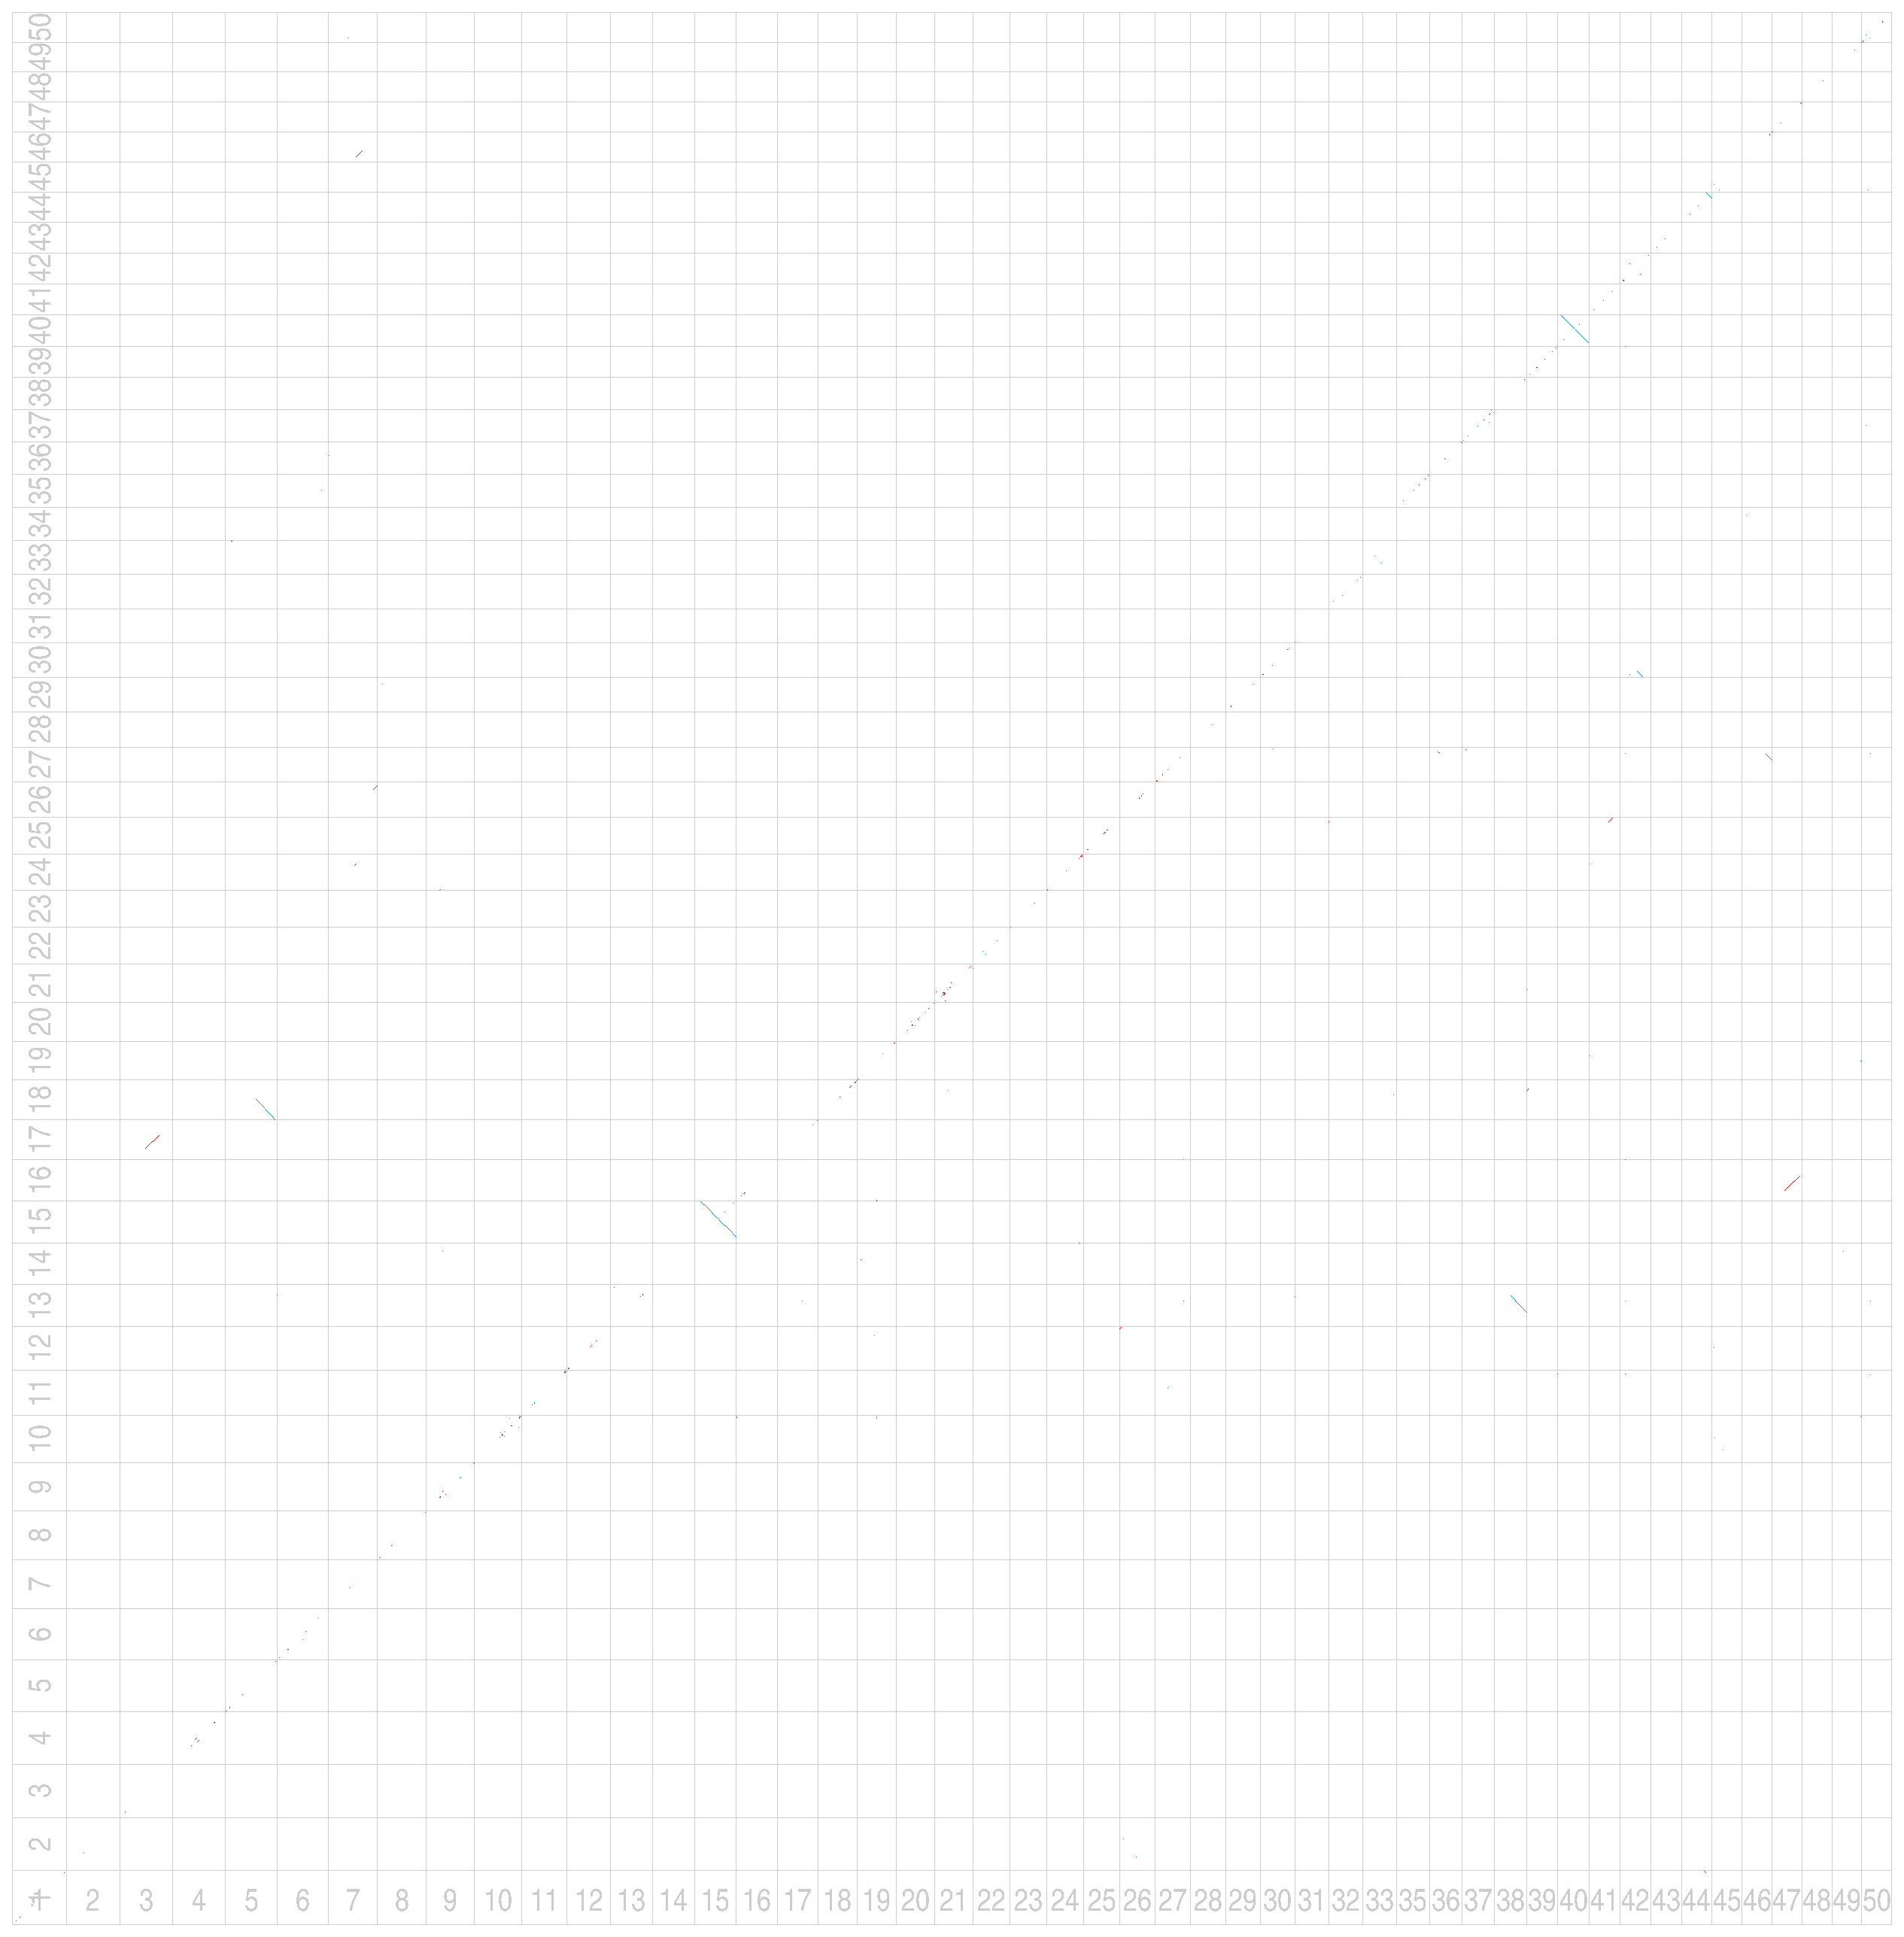
\includegraphics[width=1.1\textwidth]{figs/Adineta_Adineta.eps}
	\caption{Self-similarity of Adineta.\label{fig:Adi-Adi}}
\end{figure}

\newpage
\section{Additional Analysis}

Note that the only project has been performed locally on my personal laptop, hydra has not been used.
Yet, for this last analysis which is about the human genome, computations have been performed on Hydra that
allows more RAM that I could ever think of, i.e. 64Gb for a non prepared job running on personal session.
And as the human genome is pretty big (over 3Gb in non compressed form), its analysis require more memory
than my laptop can provide.

The human genome has been downloaded from \url{ftp://ftp.ncbi.nlm.nih.gov/genomes/all/GCA/000/001/405/GCA_000001405.15_GRCh38/seqs_for_alignment_pipelines.ucsc_ids/GCA_000001405.15_GRCh38_no_alt_analysis_set.fna.gz}\footnote{See \url{https://github.com/lh3/minimap2/issues/58}
for more details.} and \url{http://hgdownload.cse.ucsc.edu/goldenPath/hg38/chromosomes/} has been tried as well. Yet, both
these versions lead \texttt{minimap2} to crash. Therefore, only the 5 first chromosomes have been feed into \texttt{minimap2}.

Figure~\ref{fig:hg38} doesn't show anything quite useful: a given position of a chromosome is identical to the same position on the same chromosome\ldots

Yet, Figure~\ref{fig:hg38-X} is widely more complete: a humongous amount of similarities is found. It is complicated to consider all of these
to be gene copies or duplications. A hypothesis would be that human genome contains several DNA portions that are repeated, even though
these are not entire genes. These can be non-coding regions, or some recurrent motifs of proteins that have a particular function (3D shape),
making them recurrent inside the DNA sequence.

Figures~\ref{fig:hg38}~and~\ref{fig:hg38-X} were made according to the results of \texttt{minimap2} with the \texttt{asm5} preset. Figures~\ref{fig:hg38-10}
and~\ref{fig:hg38-10-X} show the same analysis but with the \texttt{asm10} preset of \texttt{minimap2}, allowing even more divergence.

\begin{figure}[!h]
	\hspace{-1cm}
	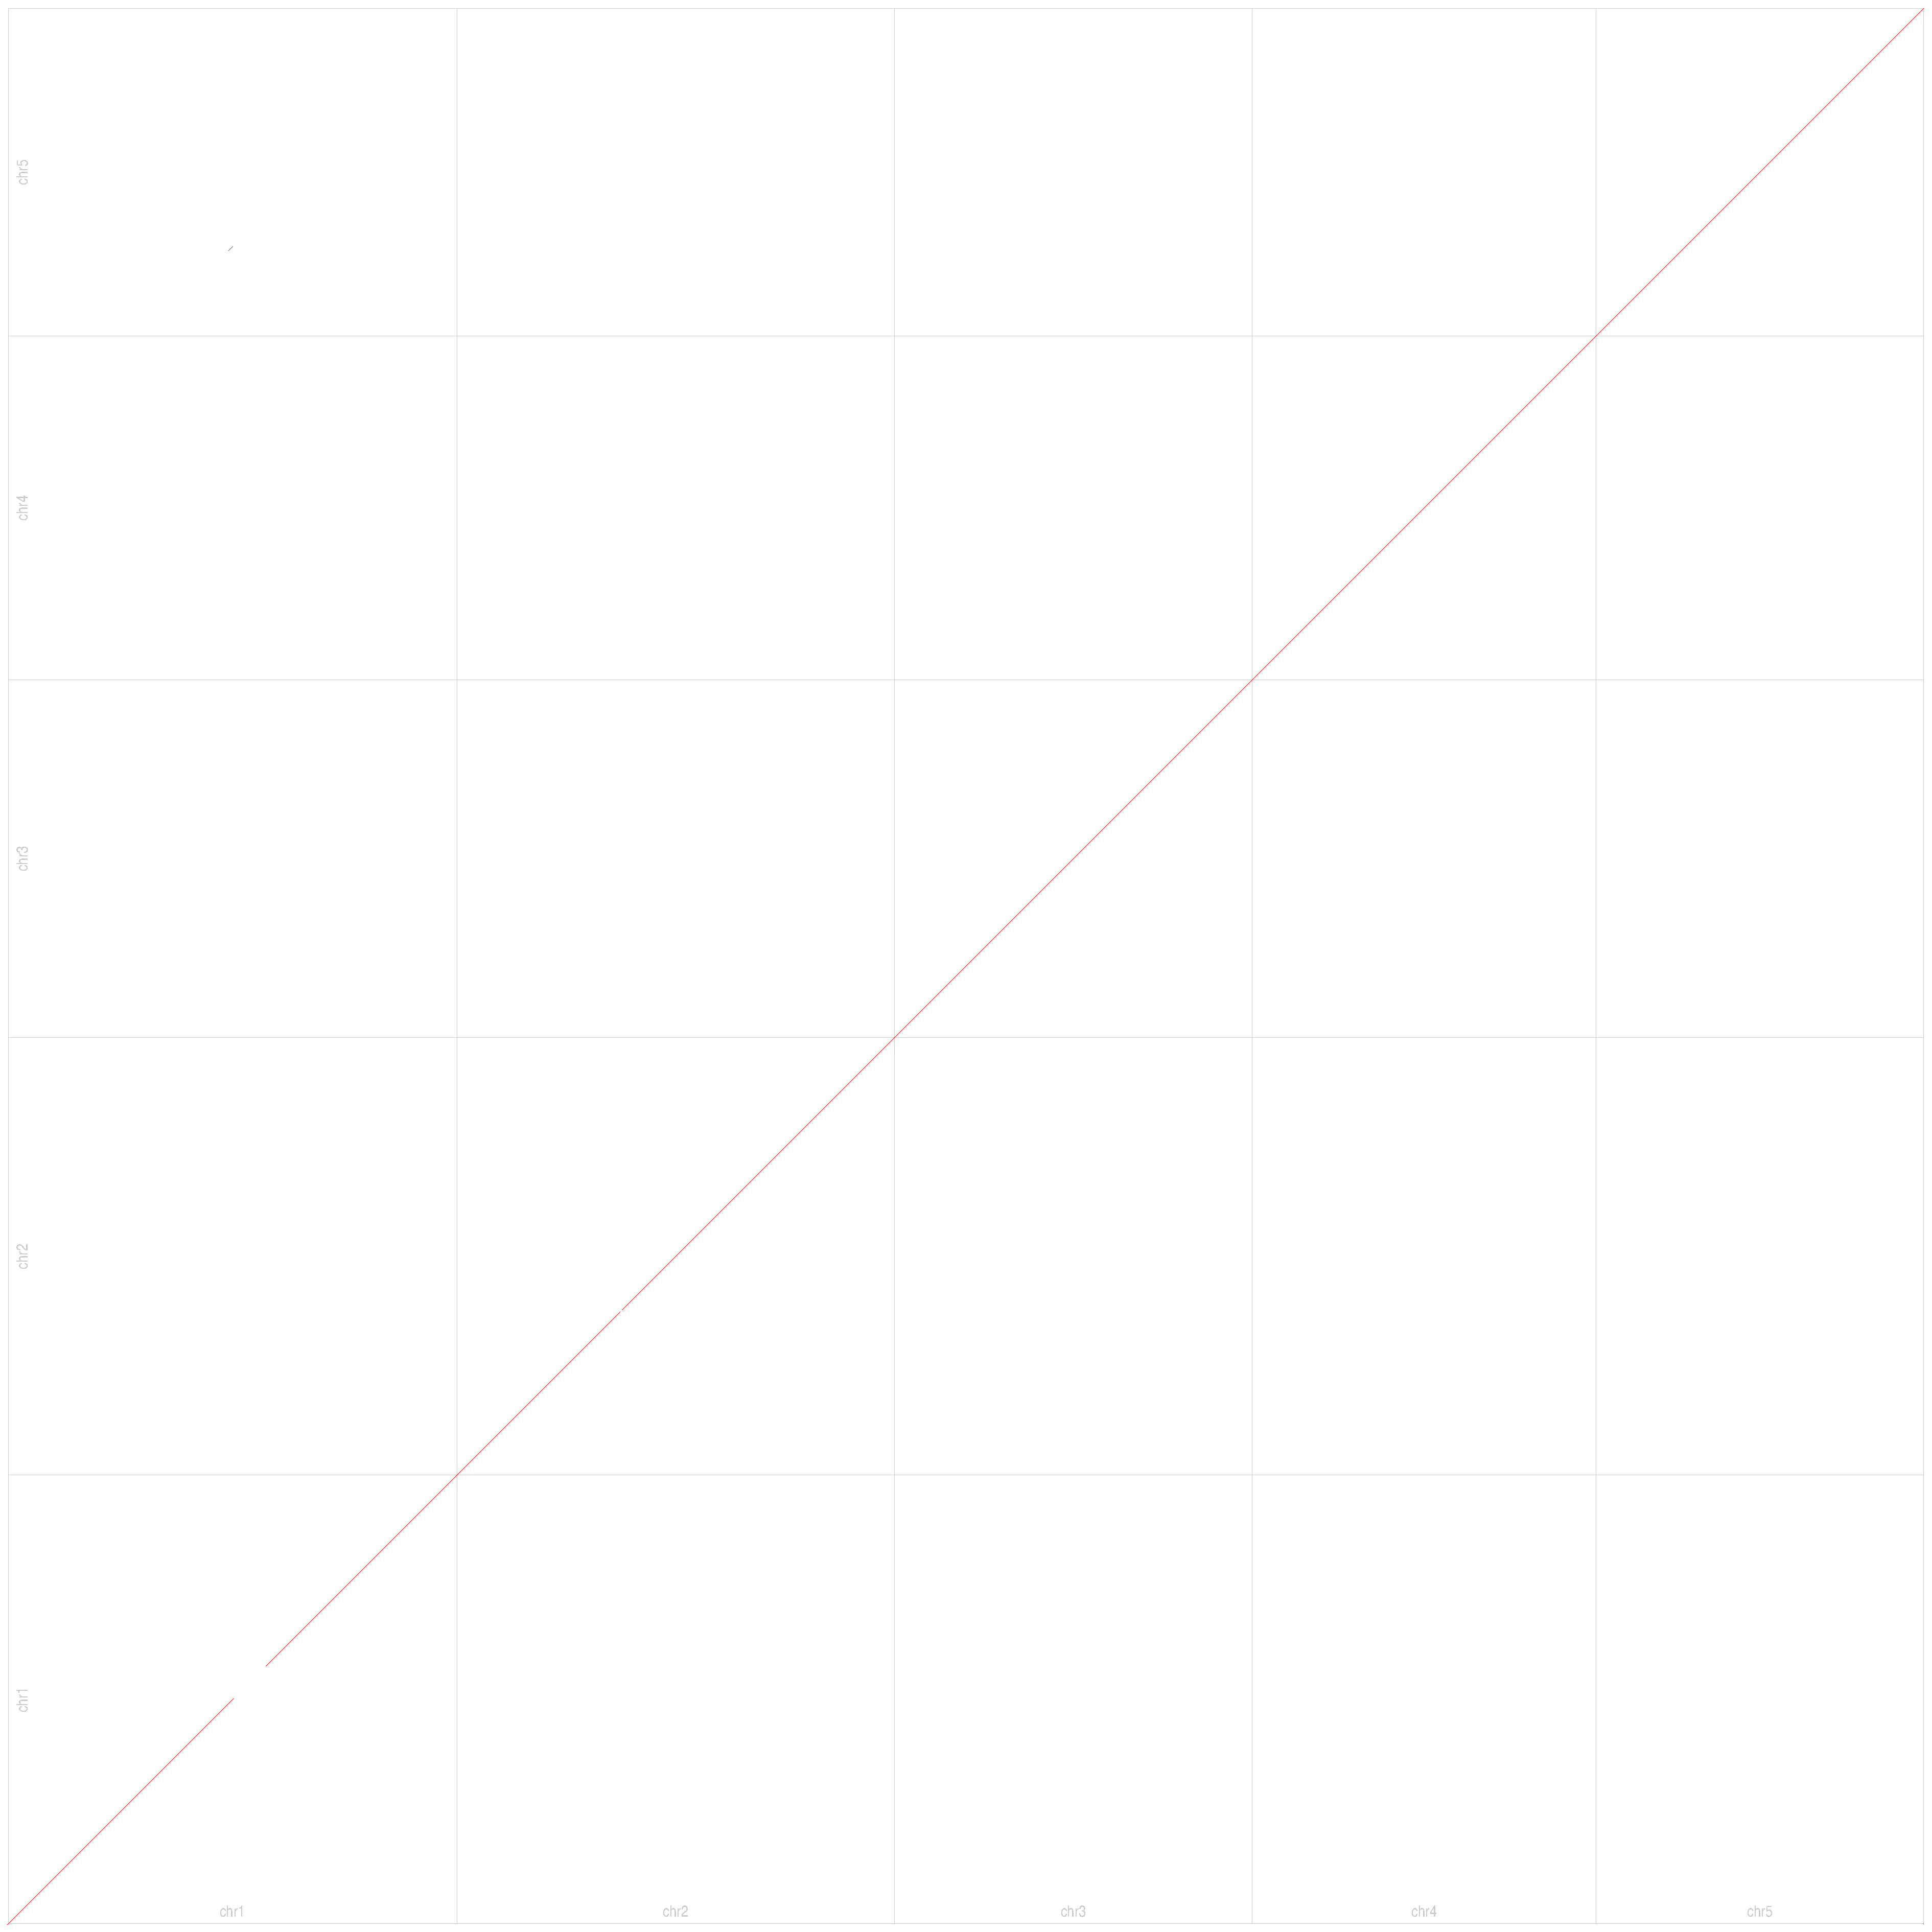
\includegraphics[width=1.1\textwidth]{figs/human.eps}
	\caption{Self-similarity \textit{asm5} of the 5 first chromosomes of the human genome (assembly hg38) without \texttt{minimap2}'s \texttt{-X} argument.
	\label{fig:hg38}}
\end{figure}

\begin{figure}[!h]
	\centering
	\includegraphics[scale=.3]{figs/x_human.jpg}
	\caption{Self-similarity \textit{asm5} of the 5 first chromosomes of the human genome (assembly hg38) with \texttt{minimap2}'s \texttt{-X} argument.
	\label{fig:hg38-X}}
\end{figure}

\begin{figure}[!h]
	\hspace{-1cm}
	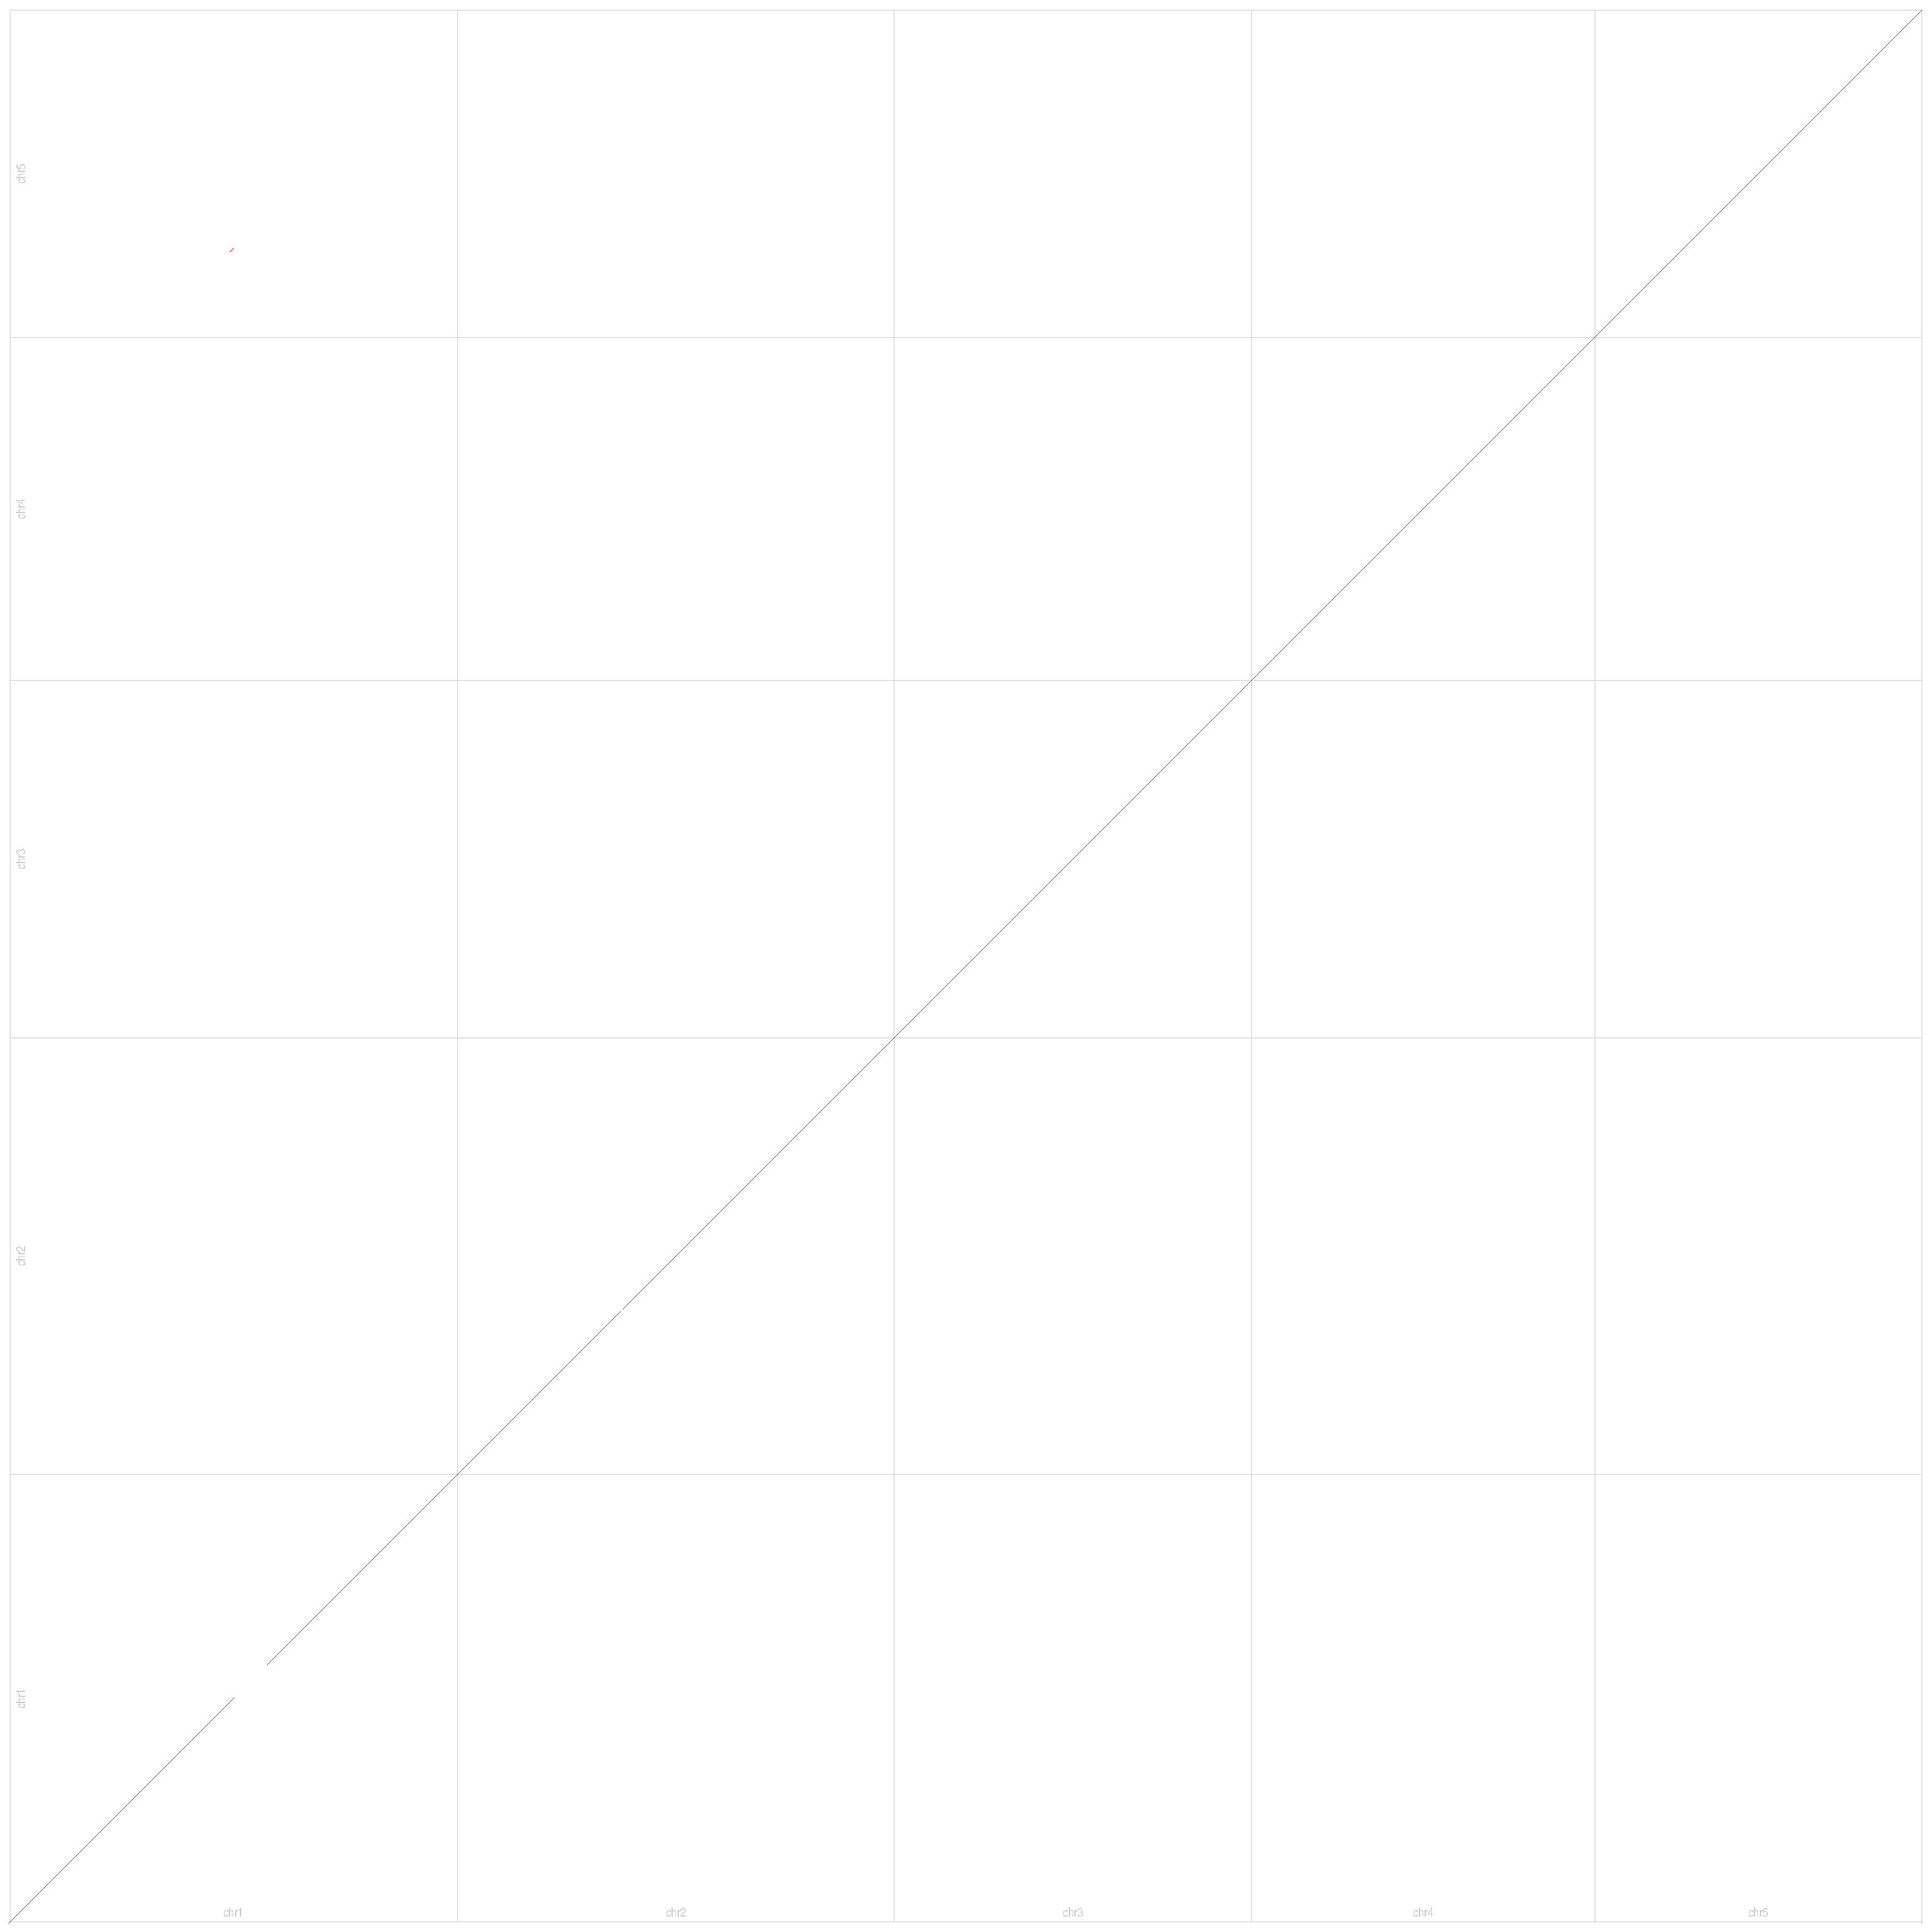
\includegraphics[width=1.1\textwidth]{figs/human_10.eps}
	\caption{Self-similarity \textit{asm10} of the 5 first chromosomes of the human genome (assembly hg38) without \texttt{minimap2}'s \texttt{-X} argument.
	\label{fig:hg38-10}}
\end{figure}

\begin{figure}[!h]
	\centering
	\includegraphics[scale=.3]{figs/x_human_10.jpg}
	\caption{Self-similarity \textit{asm10} of the 5 first chromosomes of the human genome (assembly hg38) with \texttt{minimap2}'s \texttt{-X} argument.
	\label{fig:hg38-10-X}}
\end{figure}

Figures~\ref{fig:hg38} and~\ref{fig:hg38-10} are the same, no new similarities were added by by adding the divergence threshold, and
Figures~\ref{fig:hg38-X} and~\ref{fig:hg38-10-X}, despite being too crowded are identical as well.

\end{document}
